\documentclass[numerate]{cheatsheet}
\usepackage{bm}
\usepackage{textcomp, mathcomp}
\usepackage{empheq}
\usepackage{pbox}
\usepackage{booktabs}

\lstset{style=python_style}

\doctitle{Informatik 2 Cheatsheet}
\author{Julian Lotzer – jlotzer@student.ethz.ch\\ 
Daniel Steinhauser – dsteinhauser@student.ethz.ch\\
Modified by:
Christian Leser - cleser@ethz.ch
\\ \vspace*{-0.2em}}

\begin{document}
\section{General Python} %1
	\subsection{Reference Semantics and Aliasing}
Everything is a pointer: l1 and l2 point to the same adress
\lstinputlisting{src/1_general_python/code/1_pointer_example.py}

If a copy is needed, use:
\lstinputlisting{src/1_general_python/code/1_copy_example.py}
    \subsection{Data Types}
    Python dynamically types variables, which means that the variable type can change during the program's execution
    \lstinputlisting{src/1_general_python/code/2_data_types.py}
    To convert the data type:
    \lstinputlisting{src/1_general_python/code/2_type_conversion.py}
    \subsubsection{Type Hints}
    help make code more legible
    \lstinputlisting{src/1_general_python/code/2_1_type_hints.py}
    \subsection{Input and Output}
    {\centering\underline{\textbf{Output}} \par}
    \lstinputlisting{src/1_general_python/code/3_output.py}
    {\centering\underline{\textbf{Input}} \par}
    \lstinputlisting{src/1_general_python/code/3_input.py}
    \subsection{Control Flows (if/else, while, for)}
    {\centering\underline{\textbf{if, else}} \par}
    \lstinputlisting{src/1_general_python/code/4_if_else.py}

    {\centering\underline{\textbf{while}} \par}
    \lstinputlisting{src/1_general_python/code/4_while.py}

    {\centering\underline{\textbf{for with range}} \par}
    \lstinputlisting{src/1_general_python/code/4_for_list.py}

    {\centering\underline{\textbf{for with lists}} \par}
    \lstinputlisting{src/1_general_python/code/4_for_range.py}

    \subsection{Functions}
    Functions do not have to be declared in a specific order
    \subsubsection{Function Declaration}
    \lstinputlisting{src/1_general_python/code/5_1_declaration.py}
    \subsubsection{Default arguments}
    When calling a function with default arguments, it is not necessary to call the function with arguments.
    \lstinputlisting{src/1_general_python/code/5_2_default_args.py}
    \subsubsection{Global and local variables}
    {\centering\textcolor{red}{Avoid this kind of code!} \par}
    global variables can be used within a function if declared before the funciton call. Also, local variables can be made global:
    \lstinputlisting{src/1_general_python/code/5_3_global_local.py}

\section{Algorithms} %2
    \subsection{Invariants}
The invariant is a condition in an algorithm involving a loop.\\
\begin{tabular}{l | p{0.3\linewidth} | p{0.3\linewidth}}
    Phase & Description & Example (list 'a' is sorted until index 'i')\\
    \hline \hline
    1. Initialization & the condition is met before the loop & i = 0, a[:i] = a[0] \\
    \hline
    2. Continuation & the condition holds at each iteration & i = j, a[:j] \\
    \hline
    3. Termination & the condition holds at the end of the loop & i = n, a[:n] = a[n]
\end{tabular}
    \subsection{Divide and Conquer Algorithms}
    \begin{enumerate}
        \item Divide Problem into easier to solve subproblems
        \item Solve subproblems
        \item Reassemble solutions from subproblems
    \end{enumerate}
    Examples: Sorting Algorithms for lists
    \begin{itemize}
        \item Mergesort
        \item Quick Sort
    \end{itemize}
    

\section{Python Containers} %3
    \subsection{Operations on Containers}
    Number of Elements:
\begin{lstlisting}
len(c)
\end{lstlisting}
    Contains element x?
\begin{lstlisting}
x in c
\end{lstlisting}
Iterate over all elements:
\begin{lstlisting}
for x in c:
print(x)
\end{lstlisting}
    \subsection{Sequences (ordered containers)}
    \subsubsection{Sequence Operations (Überarbeiten)} \label{section_sequence_operations}
Subscript-Operator l[i]:
\begin{lstlisting}
l = [1, 3, 'hi', -4]
print(l[2]) #output: hi
\end{lstlisting}
Enumeration:
\lstinputlisting{src/3_containers/code/2_1_enumeration.py}
Combine sequences s1 and s2 (zip):
\lstinputlisting{src/3_containers/code/2_1_zip.py}
Output with a for loop:
\lstinputlisting{src/3_containers/code/2_1_loop_output.py}
Slicing (partial sequence) of a sequence s:
\lstinputlisting{src/3_containers/code/2_1_slicing.py}
    \subsubsection{List (mutable)}
\begin{itemize}
    \item ordered data
    \item Fast Access via index
    \item Slow for updates
\end{itemize}

{\centering\underline{\textbf{Initialise a list with []}} \par}
\begin{lstlisting}
l = [1, 3, "hi", -4]
M = [[-1 for i in range(n)] for j in range(m)]
# 2D list or m x n-Matrix filled with -1
\end{lstlisting}

{\centering\underline{\textbf{Common List Operations}} \par}
\lstinputlisting{src/3_containers/code/2_2_list_operation.py}

{\centering\underline{\textbf{List Comprehension}} \par}
Apply a function $f(x)$ to all items in list l:
\begin{lstlisting}
l2 = [f(x) for x in l] #z.g. 2*x for f(x)
\end{lstlisting}
Apply a function $f(x)$ to a range:
\begin{lstlisting}
r2 = [f(x) for x in range(1,6)]
\end{lstlisting}
Apply a function $f(x)$ only to items in list l that satisfy $g(x)$ (filter):
\begin{lstlisting}
l3 = [f(x) for x in l if g(x)]
\end{lstlisting}
Example: Read a sequence of numbers:
\begin{lstlisting}
l = [int(x) for x in input("Input: ").split()]
\end{lstlisting}

\subsubsection{Sorting Algorithms for Lists} \label{section_sorting_list}
    {\centering\underline{\textbf{Selection Sort}} \par}
        \begin{minipage}{0.59\linewidth}
            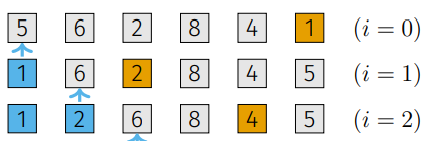
\includegraphics[width = \linewidth]{src/3_containers/images/selection_sort.png}
        \end{minipage}
        \begin{minipage}{0.39\linewidth}
            \fcolorbox{black}{cyan}{sorted list}\\
            \fcolorbox{black}{white}{unsorted list}\\
            \fcolorbox{black}{orange}{smallest value}
        \end{minipage}

        \lstinputlisting{src/3_containers/code/2_2_1_selection_sort.py}

    {\centering\underline{\textbf{Insertion Sort}} \par}
        \begin{minipage}{0.64\linewidth}
            \lstinputlisting{src/3_containers/code/2_2_1_insertion_sort.py}
        \end{minipage}
        \begin{minipage}{0.34\linewidth}
            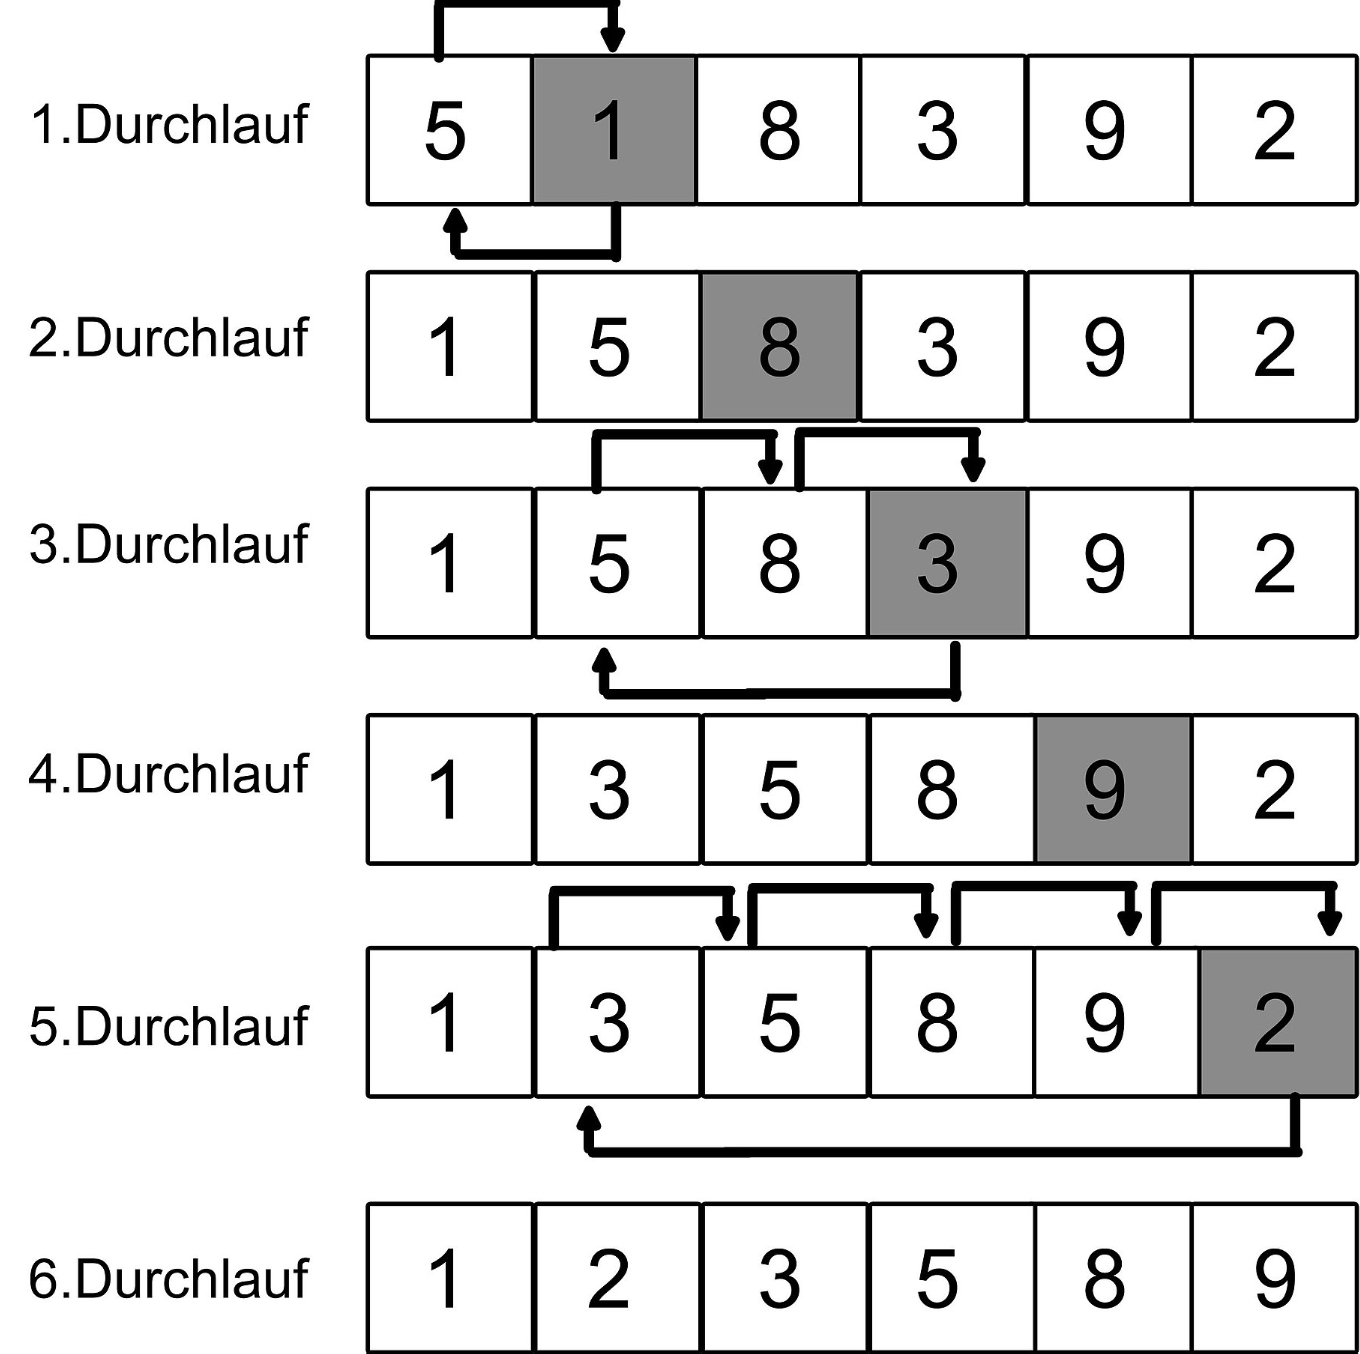
\includegraphics[width = \linewidth]{src/3_containers/images/insertion_sort.png}
        \end{minipage}

    {\centering\underline{\textbf{Bubble Sort}} \par}
        {\centering \includegraphics*[width = 0.8\linewidth]{src/3_containers/images/bubble_sort.png} \par}
        \lstinputlisting{src/3_containers/code/2_2_1_bubble_sort.py}
        
    {\centering\underline{\textbf{Mergesort (Divide and Conquer)}} \par}
        Requires $\Theta(n)$ additional storage\\
        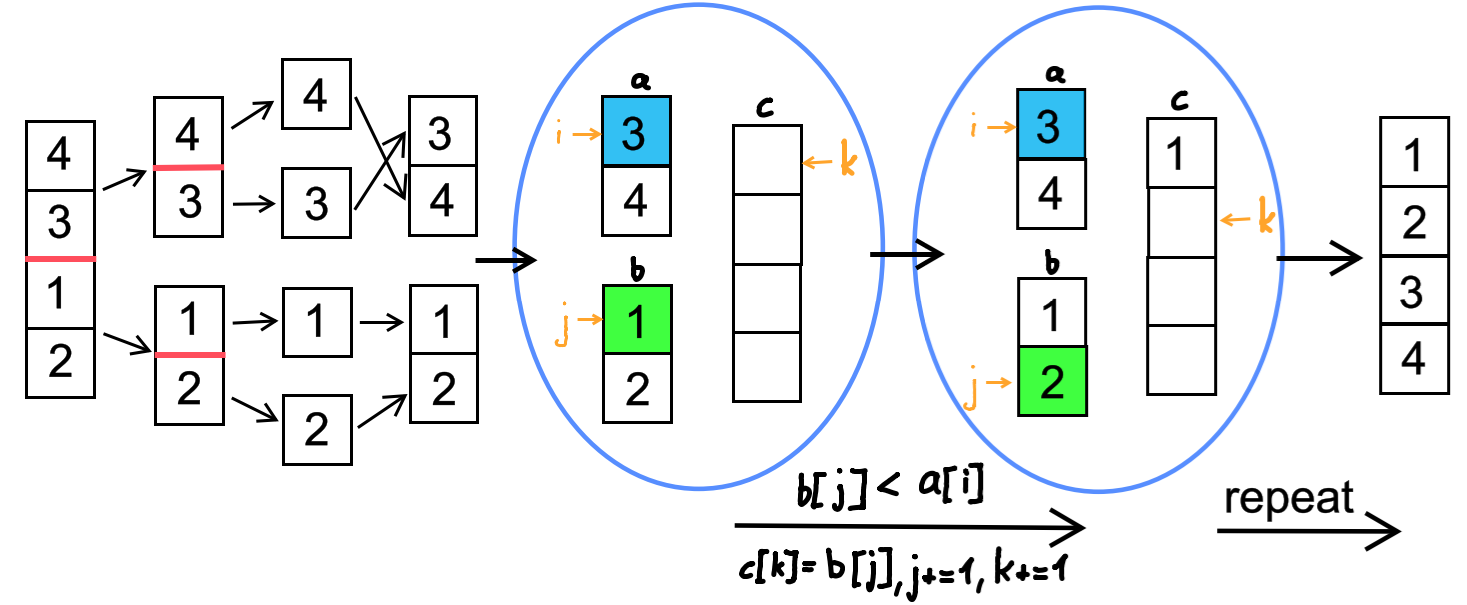
\includegraphics[width = \linewidth]{src/3_containers/images/mergesort.png}
        \fcolorbox{black}{cyan}{greater value}  \fcolorbox{black}{green}{smaller value}

        \lstinputlisting{src/3_containers/code/2_2_1_mergesort.py}
    
    {\centering\underline{\textbf{Quick Sort (Divide and Conquer)}} \par}
        Requires no additional storage\\
        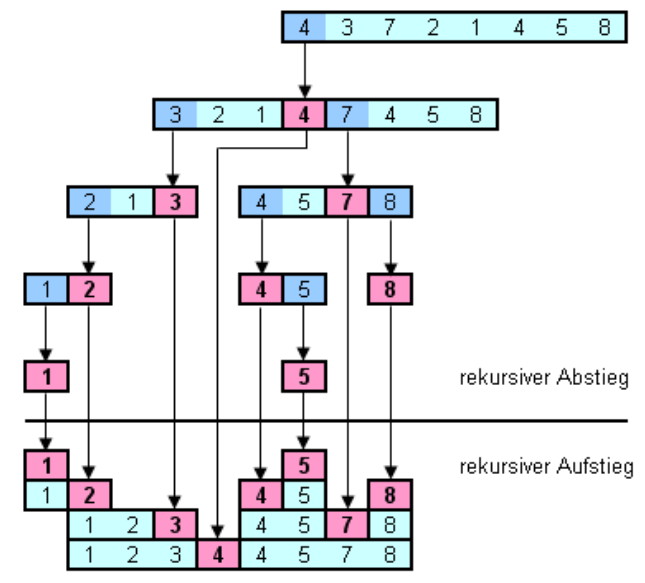
\includegraphics[width = \linewidth]{src/3_containers/images/quicksort.png}
        \fcolorbox{black}{ProcessBlue}{Pivot}  \fcolorbox{black}{CarnationPink}{Pivot is now at correct position}
        \lstinputlisting{src/3_containers/code/2_2_1_quick_sort.py}

\subsubsection{Search Algorithms for Lists}
    {\centering\underline{\textbf{Linear Search}} \par}
        \includegraphics*[width = 0.8\linewidth]{src/3_containers/images/linear_search.png}
        \lstinputlisting{src/3_containers/code/2_2_2_linear_search.py}

    {\centering\underline{\textbf{Binary Search}} \par}
        \includegraphics*[width = 0.8\linewidth]{src/3_containers/images/binary_search.png}
        \lstinputlisting{src/3_containers/code/2_2_2_binary_search.py}

    \subsubsection{Tuple (immutable)}
{\centering\underline{\textbf{Initialise a tuple with ()}} \par}
\begin{lstlisting}
t = ("a", 0, -6, 3.3)
\end{lstlisting}
    \subsubsection{Range (immutable)}
{\centering\underline{\textbf{Initialise a range}} \par}
\begin{lstlisting}
#range(start, stop, step)
#befault: start = 0, step = 1, end not included
r = range(0, 8, 2) #r ->  0   2   4   6,
\end{lstlisting}
    \subsubsection{String (immutable)}
{\centering\underline{\textbf{Initialise a string with ""}} \par}
\begin{lstlisting}
s = "hello" #s ->  'h' 'e' 'l' 'l' 'o'
#you can use both " or ' for strings 
\end{lstlisting}

{\centering\underline{\textbf{Common String Operations}} \par}
\lstinputlisting{src/3_containers/code/2_5_str_operations.py}
Example: check if s is a string with content:
\begin{lstlisting}
type(s) == str and len(s.strip()) #False if empty
\end{lstlisting}
Example: convert a string to a list of words:
\begin{lstlisting}
s = "Hello World"
w = s.split() #-> w = ['Hello', 'World']
s.split(seperator, maxsplit) 
#seperator and maxsplit are optional
#s.split() -> split at all whitespaces
#separator = ", " -> split at every ", "
#maxsplit = 10 -> split only at first 10 separators
\end{lstlisting}
    \subsection{Collections (unordered containers)}
    \subsubsection{Set (non-associative)}
{\centering\underline{\textbf{Initialise Set}} \par}
\begin{lstlisting}
s = {1, 29, 12}
\end{lstlisting}

{\centering\underline{\textbf{Common Set Operations}} \par}
\lstinputlisting{src/3_containers/code/3_1_set_operations.py}
    \subsubsection{Dictionary (associative)}
See \ref{section_sequence_operations} Sequence operations for 'enumerate' and 'zip'\\
{\centering\underline{\textbf{Initialise a Dictionary with \{\}}} \par}
A dictionary consists of \textbf{tuples (key, value)} as items. For that reason, one can think of it as a list of tuples (Which it is not in reality)
\lstinputlisting{src/3_containers/code/3_2_initialise_dict.py}

{\centering\underline{\textbf{Common Dictionary Operations}} \par}
\lstinputlisting{src/3_containers/code/3_2_dict_operations.py}

{\centering\underline{\textbf{Iterate over a Dictionary}} \par}
\lstinputlisting{src/3_containers/code/3_2_iterate_over_dict.py}

{\centering\underline{\textbf{Dictionary Comprehension}} \par}
Transform a set into a dictionary by applying $f(x)$ and $g(x)$ on every element in the set:
\begin{lstlisting}
d3 = {f(x):g(x) for x in s} #s being a set
d4 = {f(x):g(y) for x, y in z.items()} #z being a dict
\end{lstlisting}
Transform a set into a dictionary, only if the element satisfies h(x):
\begin{lstlisting}
d5 = {f(x):g(x) for x in s if h(x)}
\end{lstlisting}
Example: Multiply the value of every odd key in a dictionary by 2:
\begin{lstlisting}
d6 = {k:2*v for k, v in d.items() if k % 2 == 1}
\end{lstlisting}

\section{Python Classes} %4
    \begin{itemize}
    \item entity with a name that contains data and functionality
    \item bundling of data that belongs together contentwise
    \item definition of a new type
    \item every object of this type stores data and offers functionality
\end{itemize}

\lstinputlisting{src/4_class/code/basic_class.py}
    \subsection{Private attribute}
    \lstinputlisting{src/4_class/code/private.py}
    \subsection{Inheritance}
    \begin{itemize}
        \item Child inherits all attributes and methods from Parent
        \item Child can define additional attributes and methods
    \end{itemize}

    \lstinputlisting{src/4_class/code/inheritance.py}
    \subsection{Magical Methods}
    \begin{tabular}{c | c | c}
        Operation   & Meaning               & Magical Method\\
        \hline \hline
        $<$         & Less than             & \_\_lt\_\_\\
        $<$=        & Less than or equal    & \_\_le\_\_\\
        $>$         & Greater than          & \_\_gt\_\_\\
        $>$=        & Greater than or equal & \_\_ge\_\_\\
        ==          & Equal to              & \_\_eq\_\_\\
        !=          & Not equal to          & \_\_ne\_\_\\
        +, +=       & Addition              & \_\_add\_\_, \_\_iadd\_\_\\
        -           & Subtraction           & \_\_sub\_\_\\
        *           & Multiplication        & \_\_mul\_\_\\
        /           & Division              & \_\_truediv\_\_\\
        //          & Integer division      & \_\_floordiv\_\_\\
        \%          & Modulo                & \_\_mod\_\_\\
        **          & Exponentiation        & \_\_pow\_\_\\
        print()     & overload print()      & \_\_str\_\_\\
        -           & Negation              & \_\_neg\_\_
    \end{tabular}

\section{Data Structures} %4 -> 5
    \subsection{FIFO / LIFO}
    FIFO - first in, first out, fast access to first inserted element
    {\centering 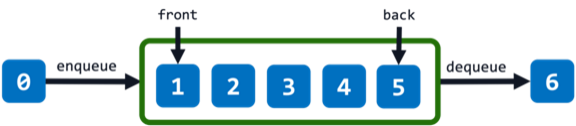
\includegraphics[width = 0.8\linewidth]{src/4_data_structure/images/fifo.png} \par}
    LIFO - last in, first out, fast access to last inserted element
    {\centering 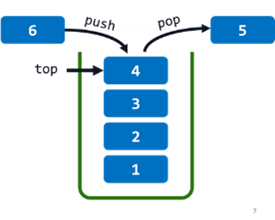
\includegraphics[width = 0.5\linewidth]{src/4_data_structure/images/lifo.png} \par}
    \subsection{Binary Search Tree (BST)}
    
    \subsubsection{(Max) Heaps}
    Heaps are only visualised as trees while they are stored as arrays\\
    Useful for quick access to max (/ min) value
    \begin{itemize}
        \item complete binary tree (see \ref{sec_tree_terminology} Tree terminology)
        \item Key of parent is always greater (smaller) than the one of its children
    \end{itemize}
    \begin{minipage}{0.49\linewidth}
        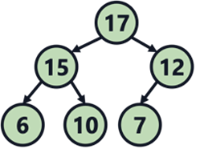
\includegraphics[width = 0.95\linewidth]{src/5_data_structure/images/max_heap.png}
    \end{minipage}
    \begin{minipage}{0.49\linewidth}
        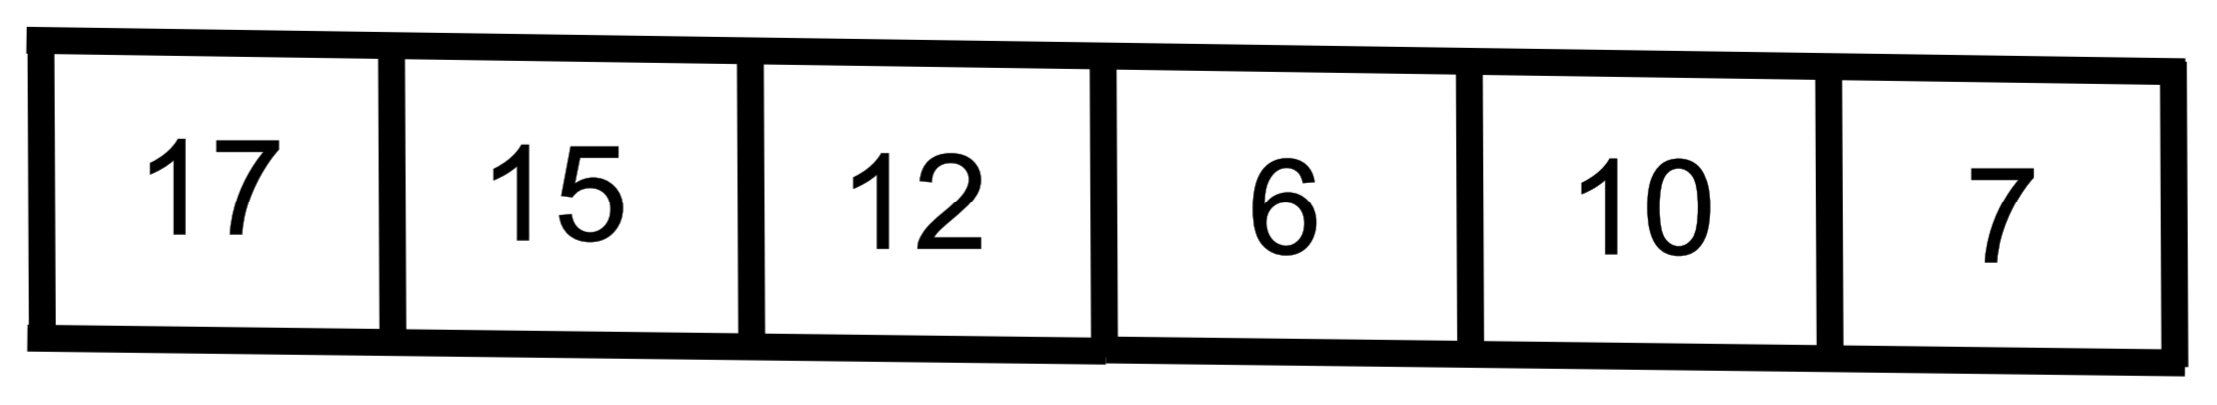
\includegraphics[width = 0.95\linewidth]{src/5_data_structure/images/max_heap_array.png}
        Array corresponding to the max heap
    \end{minipage}

    {\centering\underline{\textbf{Implementation}} \par}
        Heap[i = 1] = Root:\\
        \begin{itemize}
            \item Children of i: {2i+1, 2i+2}
            \item Parent of i: i-1//2
        \end{itemize}

    {\centering\underline{\textbf{Height}} \par}
        $H(n) = \log_2(n+1)$
        \begin{lstlisting}
# a is a heap with n elements
def height(a):
    return math.log(len(a) + 1, 2)
        \end{lstlisting}

    {\centering\underline{\textbf{Sift Up}} \par}
        Reestablishes Heap structure, Used in 'Insert'
        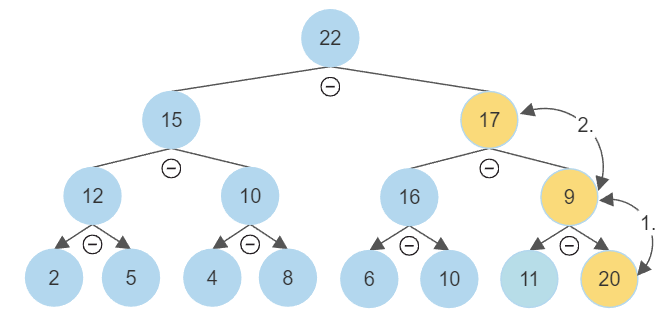
\includegraphics[width = \linewidth]{src/5_data_structure/images/heap_sift_up.png}
        \lstinputlisting{src/5_data_structure/code/heap_sift_up.py}

    {\centering\underline{\textbf{Sift Down}} \par}
        Reestablishes Heap structure, Used in 'Remove' and 'Heapify'\\
        If the parent value is smaller: exchange the parent value with the greater children value
        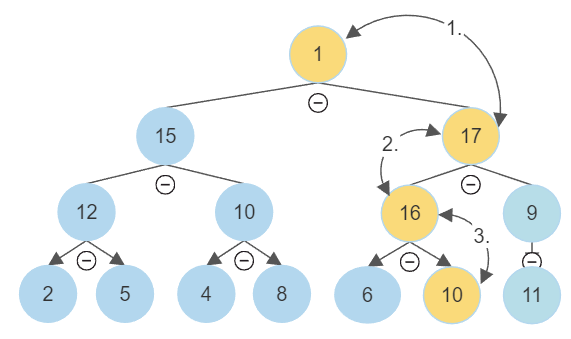
\includegraphics[width = \linewidth]{src/5_data_structure/images/heap_sift_down.png}
        \lstinputlisting{src/5_data_structure/code/heap_sift_down.py}

    {\centering\underline{\textbf{Insert}} \par}
        \lstinputlisting{src/5_data_structure/code/heap_insert.py}

    {\centering\underline{\textbf{Remove Max Value}} \par}
        Change the first and last entry in the array, then delete the last entry. Now, the max value does not exist any more.
        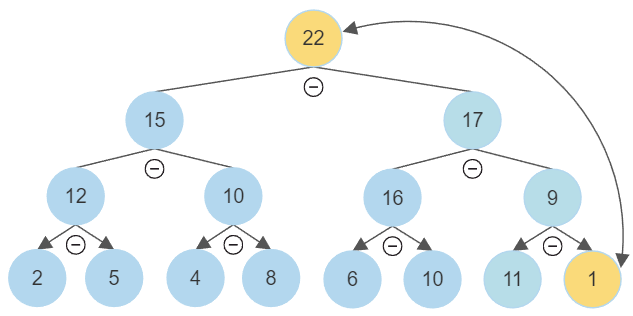
\includegraphics[width = \linewidth]{src/5_data_structure/images/heap_remove_max.png}
        Reestablish the Heap condition by applying Sift Down.
        \lstinputlisting{src/5_data_structure/code/heap_remove_max.py}

    {\centering\underline{\textbf{Heap creation / Heapify}} \par}
        Repeatedly apply Sift Down until the array is heapified.\\
        Leaves fulfill the heap condition trivially $\rightarrow$ only “heapify” the first n/2 elements.
        \lstinputlisting{src/5_data_structure/code/heap_heapify.py}

    {\centering\underline{\textbf{Sorting a heap}} \par}
        If "a" is a heap, one can efficiently sort the array:
        \lstinputlisting{src/5_data_structure/code/heap_sort.py}
    

    \subsection{Linked List}
    \begin{itemize}
        \item ordered data
        \item fast updates in first elements
    \end{itemize}
    \includegraphics*[width = 0.9\linewidth]{src/4_data_structure/images/linked_list.png}

    {\centering\underline{\textbf{Implementation}} \par}
        \lstinputlisting{src/4_data_structure/code/llist_implementation.py}

    {\centering\underline{\textbf{Traversal}} \par}
        \lstinputlisting{src/4_data_structure/code/llist_traversal.py}

    {\centering\underline{\textbf{Search}} \par}
        \lstinputlisting{src/4_data_structure/code/llist_search.py}

    {\centering\underline{\textbf{Insert}} \par}
        \lstinputlisting{src/4_data_structure/code/llist_insert.py}

    {\centering\underline{\textbf{Remove}} \par}
        \lstinputlisting{src/4_data_structure/code/llist_remove.py}
    
    {\centering\underline{\textbf{Convert List to Linked List}} \par}
        \lstinputlisting{src/4_data_structure/code/llist_list_to_llist.py}
    \subsection{Hash Tables}
    \begin{minipage}{0.49\linewidth}
        \begin{itemize}
            \item fast access to elements
            \item Unsorted, unordered data
            \item $\mathcal(O)$ only in expectation
        \end{itemize}
        Given an element 'x' to be stored, a Hash Table 'M' of length 'l' and a hash function 'f(x)':
        \begin{lstlisting}
M[f(x) % l] = x
\end{lstlisting}
    \end{minipage}
    \begin{minipage}{0.49\linewidth}
        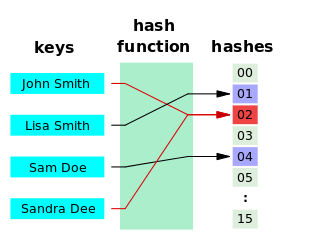
\includegraphics[width = 0.95\linewidth]{src/5_data_structure/images/hash_function.png}
        \textcolor{red}{example of collision}
    \end{minipage}

    \subsubsection{Collision handling}
        Entry at calculated index may already contain an element
        \begin{tabular}{p{0.45\linewidth} | p{0.45\linewidth}}
            \hline
            Probing: next available index is chosen & Chaining: a linked list at every entry\\
            \hline
            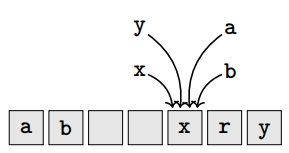
\includegraphics[width = \linewidth]{src/5_data_structure/images/probing.png} & 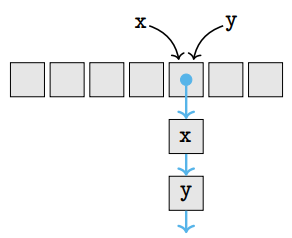
\includegraphics[width = \linewidth]{src/5_data_structure/images/chaining.png}
        \end{tabular}

    \subsection{Quadtree}
    \begin{itemize}
        \item Faster searching for points within a rectangle
        \item Efficient for querying multiple rectangles
    \end{itemize}
    Data containing two values are inserted into squares. The squares have a maximum number of points they may contain. If a new point would exceed that limit, the square is subdivided into four smaller squares.\\
    {\centering 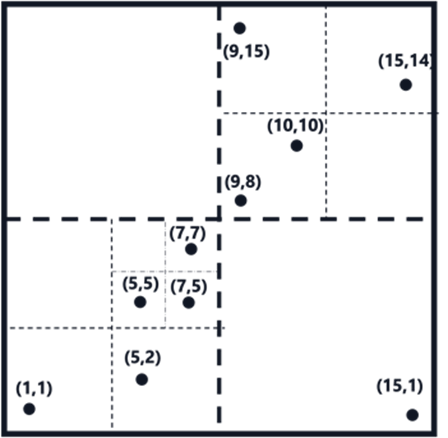
\includegraphics[width = 0.5\linewidth]{src/4_data_structure/images/quadtree.png} \par}

    {\centering\underline{\textbf{Implementation}}\par}
        \lstinputlisting{src/4_data_structure/code/quad_implementation.py}

    {\centering\underline{\textbf{Insert}}\par}
        {\centering 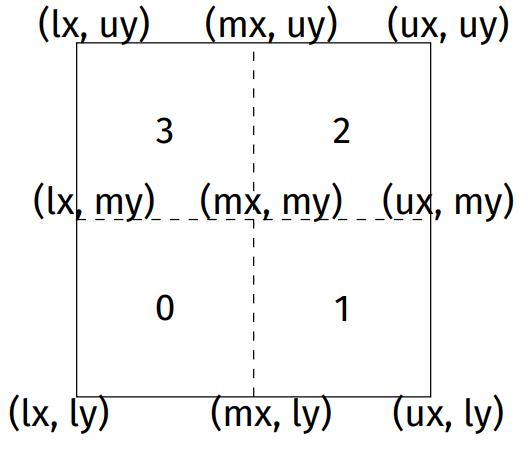
\includegraphics[width = 0.6\linewidth]{src/4_data_structure/images/quad_divide.png} \par}
        \lstinputlisting{src/4_data_structure/code/quad_insert.py}
    
    {\centering\underline{\textbf{Search}}\par}
        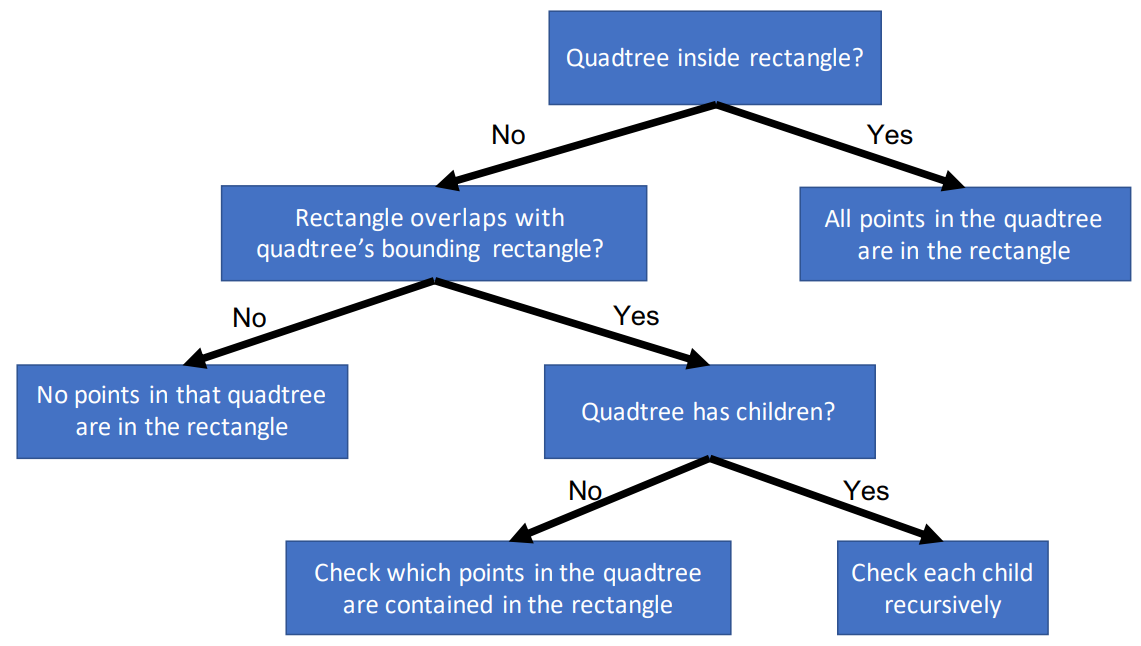
\includegraphics[width = \linewidth]{src/4_data_structure/images/quadtree_rectangle.png}
        \lstinputlisting{src/4_data_structure/code/quad_search.py}
    

\section{Runtime analysis} %5 -> 6
    \subsection{Runtime analysis}

\section{Programming Concepts} %6 -> 7
    \subsection{Compiled vs Interpreted}
Compiled (C++):
\begin{itemize}
    \item Program code is translated to assembly.
    \item Assembly is executed.
    \item Single translation, with optimizations.
    \item Usually, higher performance
\end{itemize}
Interpreted (Python):
\begin{itemize}
    \item Program code executed together with translation.
    \item Translation is repeated each time.
    \item Quick and easy to make minor changes.
\end{itemize}


    \subsection{Static vs Dynamically Typed}
C++ is statically typed:
\begin{itemize}
    \item Each element has a type defined by the programmer.
    \item Types used fitting together correctly is checked at compilation, yielding compile time errors (happen during the program itself) if wrong.
\end{itemize}
Python is dynamically typed:
\begin{itemize}
    \item Elements have no type in advance.
    \item At runtime the type is chosen.
    \item Type changeable at runtime.
    \item Depending on the type when executing, there may be runtime errrors (happen during the program).
    \item Errors are more difficult to debug, do not happen all the time.
\end{itemize}

    \subsection{Generic Programming}
The goal of generic programming is to make code as widely usable as possible (no need for new functions for different types).

Can be done with templates in C++.

No need to do anything in Python thanks to dynamic typing.
    \subsection{Functional programming}
    Pass functions as parameters to functions.
    Example:
    \lstinputlisting{src/6_programming_concepts/code/functional_example.py}

    \subsubsection{Lambda Expressions}
        Lambda functions are small functions without a specific name, useful to pass into a function as parameter.
        \lstinputlisting{src/6_programming_concepts/code/lambda.py}
    
    \subsubsection{Common Functions}
        {\centering \underline{\textbf{Map}} \par}
        • map(func, it) – applies a function on each element of a container.
        \lstinputlisting{src/6_programming_concepts/code/map.py}
        {\centering \underline{\textbf{Filter}} \par}
        • filter(func, it) – removes any elements that don’t fulfil a condition.
        \lstinputlisting{src/6_programming_concepts/code/filter.py}
        {\centering \underline{\textbf{Reduce}} \par}
        • reduce(func,it) – recursively reduce a container to a single value by applying a function to two elements.
        \lstinputlisting{src/6_programming_concepts/code/reduce.py}
        

\section{Dynamic Programming (DP)} %7 -> 8
    \begin{itemize}
    \item “bottom-up” strategy
    \item iteratively solve smaller problems to solve progressively bigger problems
    \item Overlapping subproblems
    \item answers to smaller problems are stored in a table
    \item Example: Fibonacci
\end{itemize}

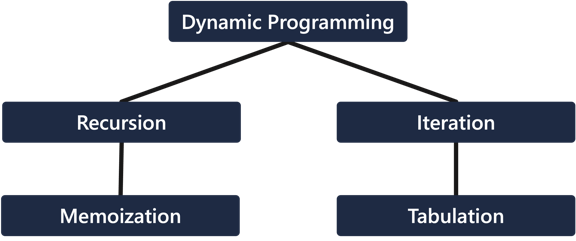
\includegraphics[width = \linewidth]{src/7_dp/images/dp.png}

Convert code from recursive to dynamic programming:
\begin{itemize}
    \item Look for repeating subproblems
    \item look for an optimal substructure to the solution – how does the answer of the problem depend on the answer of the subproblems?
    \item Should the answers of the subproblems be stored in a list? A table?
    \item Flip the recursive implementation around to implement a bottom-up, iterative solution.
\end{itemize}

{\centering \underline{\textbf{Example: dynamic programming approach to Fibonacci}} \par}
\lstinputlisting{src/7_dp/code/fibonacci.py}


\section{Machine Learning (ML)} %8
    create functions which map inputs to desired outputs by analysing underlying patterns
\begin{itemize}
    \item Regression: find output value $\in \mathbb{R}$ based on input. Example: given a house has 5 bedrooms, 1000 square meters, what is its price?
    \item Classification: assign element to a group. Example: Based on color and texture, is a mushroom edible?
\end{itemize}

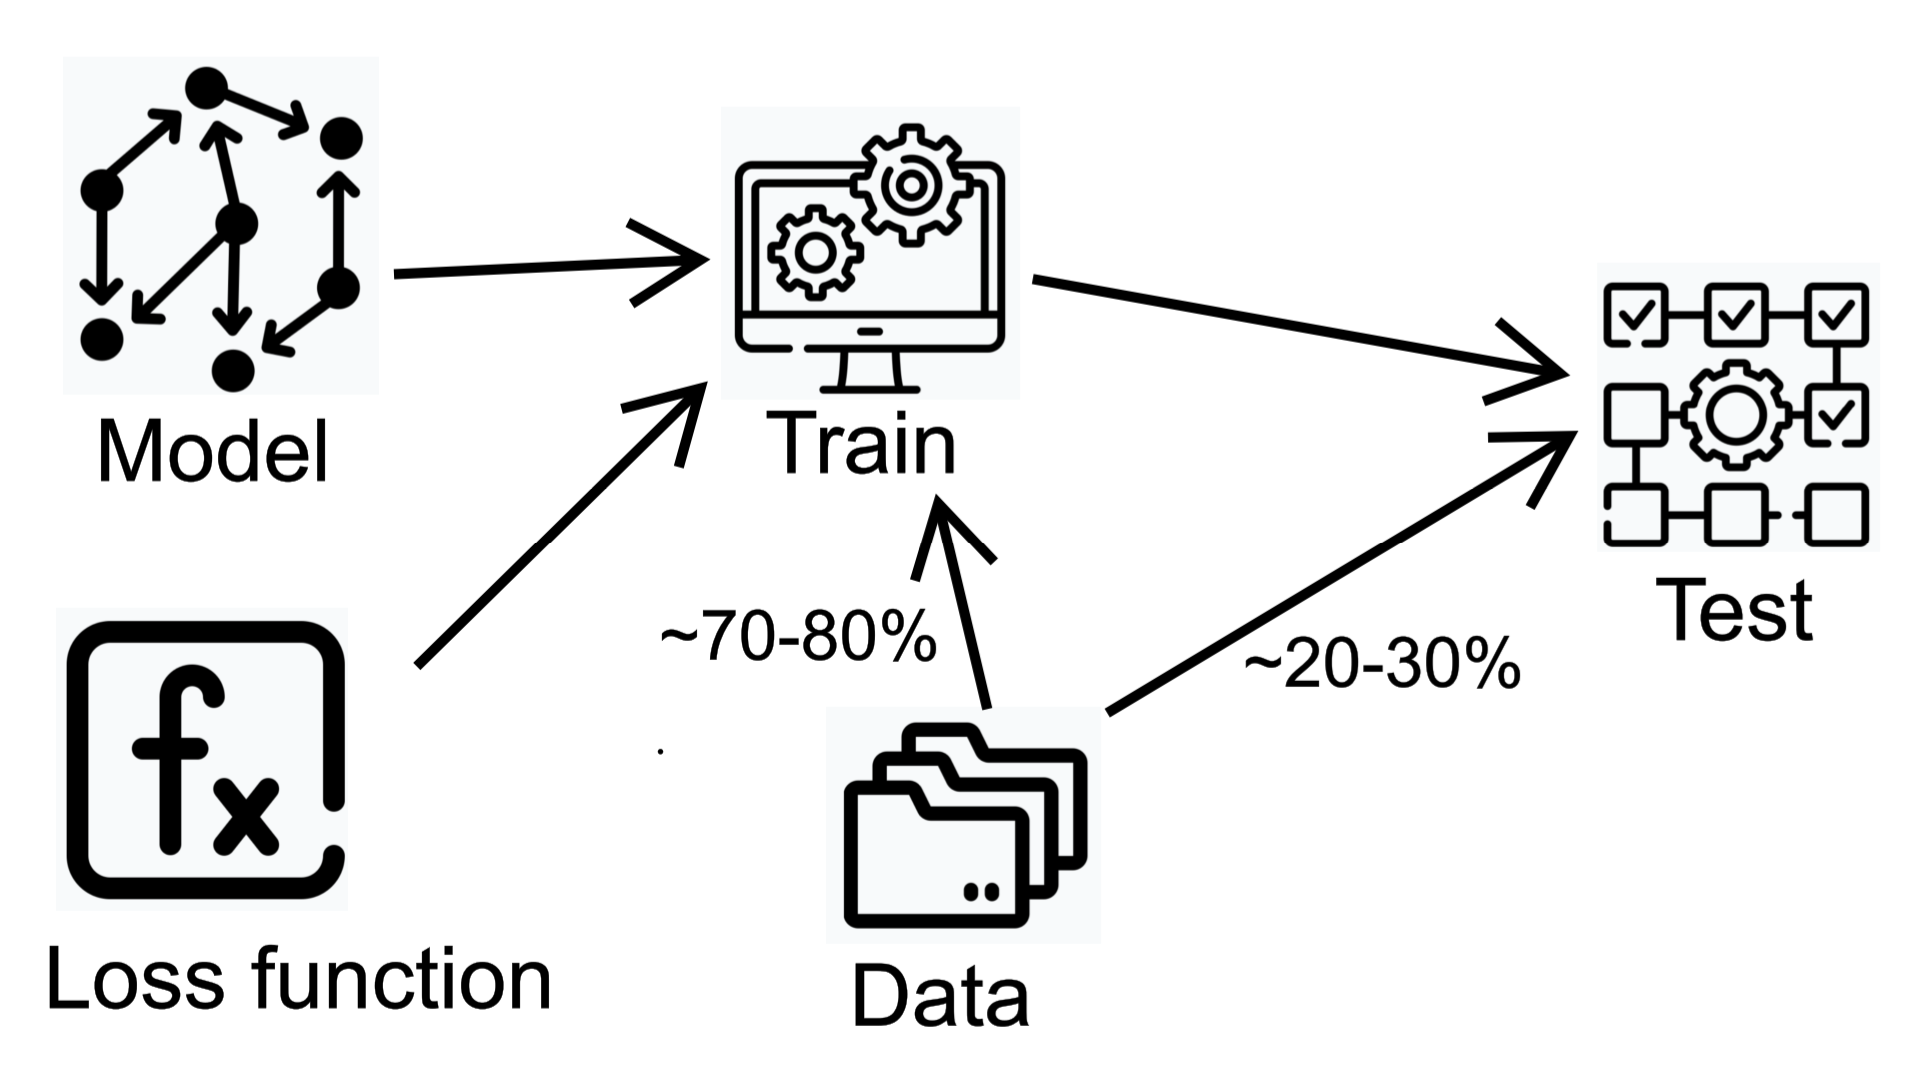
\includegraphics[width = \linewidth]{src/8_ml/images/ml_overview.png}
\lstinputlisting{src/8_ml/code/ml_example.py}

Loss function:
\begin{itemize}
    \item $\frac{\text{\# wrongly classified examples}}{\text{\# total examples}}$
    \item Mean Square Error (MSE)
    \item L2 (Gauss Loss)
\end{itemize}

\section{Numpy} %9
    Numpy is a Python package (equivalent to a C++ library) which supports operations with n-dimensional arrays and various computational methods.

Import the Numpy package:
\begin{lstlisting}
import numpy as np
\end{lstlisting}

Now you can refer to functions/classes from Numpy using: "np".

    \subsection{Python Lists vs. Numpy Arrays}
Numpy arrays are like Python lists. Below is a summary of the key differences.
\begin{tabular*}{\linewidth}{m{0.44\linewidth} | m{0.44\linewidth}}
    Python Lists & Numpy Arrays\\
    \hline
    Variable size & Fixed size\\
    \hline
    Different element types & Single element type\\
    \hline
    Mathematical operations on single elements only & Mathematical operations on whole arrays\\
    \hline
    Primarily 1D & Multi-dimensional\\
\end{tabular*}

    \subsection{Declaring Numpy Arrays}
{\centering\underline{\textbf{Using sequences}} \par}
\lstinputlisting{src/9_numpy/code/3_sequence.py}

{\centering\underline{\textbf{Using random numbers}} \par}
\lstinputlisting{src/9_numpy/code/3_random.py}

{\centering\underline{\textbf{Using arange command}} \par}
creates an array from the start to the stop value with a given step value, stop is \textbf{not} inclusive
\lstinputlisting{src/9_numpy/code/3_arange.py}

{\centering\underline{\textbf{Using linspace command}} \par}
creates a numpy array with num equally spaced elements between start and stop, stop is inclusive:
\lstinputlisting{src/9_numpy/code/3_linspace.py}
    \subsection{Numpy Array operations}
{\centering\underline{\textbf{Common numpy array operations}} \par}
\lstinputlisting{src/9_numpy/code/4_common_operations.py}
To access lines of a 2D array, see slicing.

{\centering\underline{\textbf{Slicing}} \par}
{\centering\textbf{stop is not included} \par}
\begin{itemize}
       \item 1D array: $A[\text{start}:\text{stop}:\text{step}]$
\end{itemize}
\begin{lstlisting}
A = np.arange(10) #array([0,1,2,3,4,5,6,7,8,9])
A[2:5:2] #array([2,4])
\end{lstlisting}

\begin{itemize}
       \item 2D array: $A[\underbrace{\text{start}:\text{stop}}_{\text{row}}, \underbrace{\text{start}:\text{stop}}_{\text{column}}]$
\end{itemize}
default values: start = 0, stop = len(A)
if only one number is given, only the row / column corresponding to that index is taken
\begin{lstlisting}
A = np.array([[1,2,3],[4,5,6],[7,8,9]])
A[1,:] #array([4,5,6]) #row at index 1
A[:,2] #array([3,6,9]) #column at index 2
A[0:2,1:3] #array([2,3],[5,6]) # rows 0 and 1, columns 1 and 2
\end{lstlisting}

{\centering\underline{\textbf{Statistics}} \par}
\lstinputlisting{src/9_numpy/code/4_statistics.py}

{\centering\underline{\textbf{Mathematical Operations}} \par}
Most mathematical operations are carried out element-wise:
\lstinputlisting{src/9_numpy/code/4_math_operations.py}

{\centering\underline{\textbf{Filtering}} \par}
\lstinputlisting{src/9_numpy/code/4_filter.py}

\section{Pandas} %10
    Pandas is a Python package which supports working with tabulated data.

To import pandas, use:
\begin{lstlisting}
import pandas as pd
\end{lstlisting}

Now you can refer to classes and functions from the package using ”pd”.
    \subsection{read CSV file into dataframe}
\begin{lstlisting}
climate = pd.read_csv("climate.csv", sep=",", index_col=0, usecols=["time", ...])
#"sep" -> what characters values in the csv file are separated by. "index_col" -> what the index column will be. "usecols" -> what columns of the csv data will be #selected.
\end{lstlisting}
    \subsection{Pandas Dataframe operations}
A dataframe can be thought of as a list within a list supporting access in more meaningful ways compared to using indices.

\begin{tabular*}{\linewidth}{m{0.45\linewidth} | m{0.45\linewidth} |}
    \textbf{Example dataframe} & \textbf{Change Index Column}\\
    \hline
    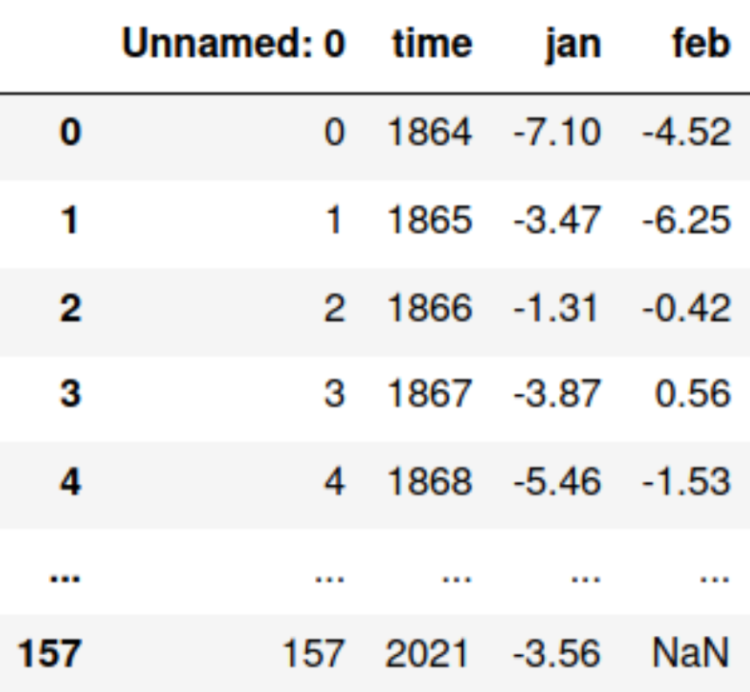
\includegraphics[width=\linewidth]{src/10_pandas/images/pd_dataframe_index.png} & 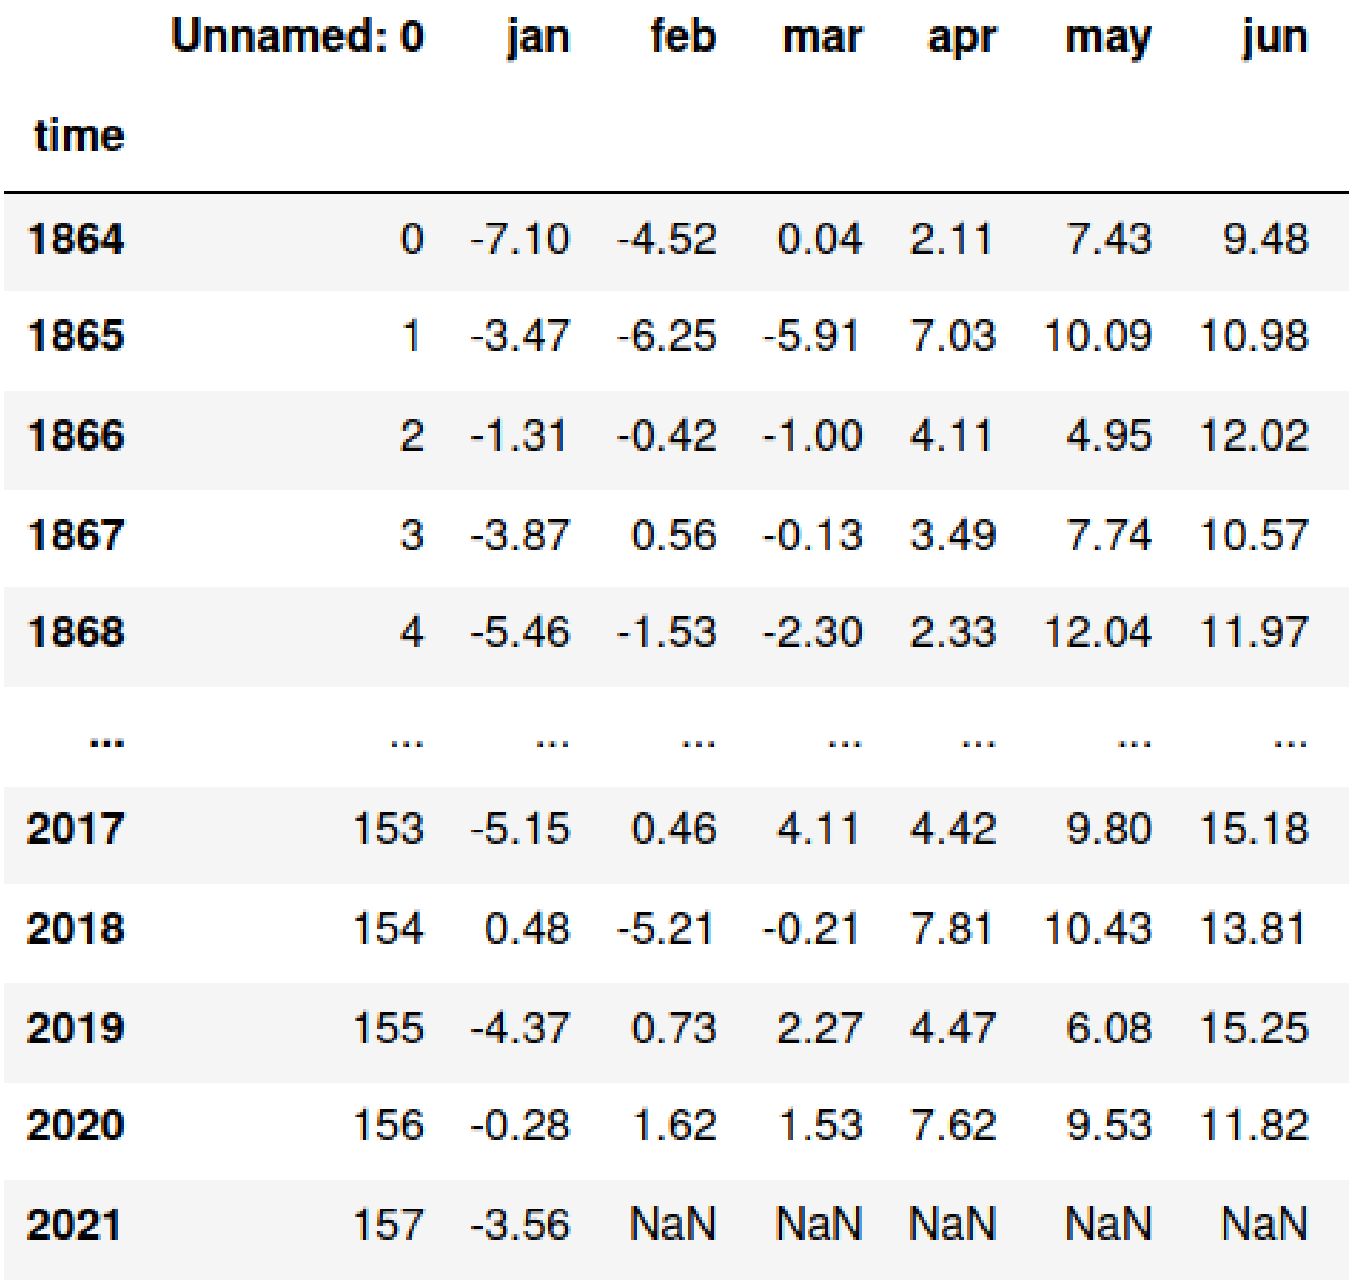
\includegraphics[width = 0.8\linewidth]{src/10_pandas/images/pd_dataframe_time.png}\\
    table of the climate, entries accessible via index. The leftmost column is known as the "index column". & \lstinputlisting{src/10_pandas/code/change_index.py} table of the climate, entries accessible via time
\end{tabular*}
 
{\centering\underline{\textbf{Rename Columns}} \par}
\begin{lstlisting}
climate = climate.rename(columns={"old_index_name":"new_index_name", ...})
#renames the "old_index_name" column to "new_index_name"
\end{lstlisting}
rename all columns (len(data.columns) = number of colums must be true)
\begin{lstlisting}
data.columns = ["Date", "January", "February", ...]
\end{lstlisting}

{\centering\underline{\textbf{Access Dataframe Elements}} \par}
\lstinputlisting{src/10_pandas/code/access_elements.py}

{\centering\underline{\textbf{Filter Dataframes}} \par}
Filter rows:
\begin{lstlisting}
climate[climate["jan"]>2]
#filters out the rows with values in the "jan" column #less than 2
\end{lstlisting}
• Example: All entries in "jan" with values more than 2:
\begin{lstlisting}
climate["jan"][climate["jan"]>2]
\end{lstlisting}

{\centering\underline{\textbf{Dealing with Invalid Data}} \par}
Convert all the values in a column to numeric:
\begin{lstlisting}
data[column] = pd.to_numeric(data[column], errors="coerce")
#converts all the values to numeric values. #errors="coerce" -> converts values which cannot be #converted to NaN.
\end{lstlisting}
Delete all rows containing NaN entries:
\begin{lstlisting}
data.dropna(axis = 0, how="any")
#how="any" -> delete row if any value is NaN.
#how="all" -> delete row if all values are NaN
#axis = 1 -> delete column instead of row
\end{lstlisting}
• Fill all entries containing NaN with a value:
\begin{lstlisting}
data.fillna(0) #fill any NaN entries with 0
\end{lstlisting}

{\centering\underline{\textbf{Modify Dataframes}} \par}
Add a column:
\begin{lstlisting}
climate["new_col"] = climate["time"] + climate["jan"] 
#"new_col" is a new column whose values are #those of the "time" and "jan" column added
\end{lstlisting}
Delete a column:
\begin{lstlisting}
climate = climate.drop(columns=["time"])
#delete the "time" column
\end{lstlisting}
Add a row:
\begin{lstlisting}
d = {"mar":34, "jan":23}
climate.append(d, ignore_index=True)
#adds another row with the values 34 for "mar" and 23 for #"jan". Other entries are NaN
\end{lstlisting}
Delete a row:
\begin{lstlisting}
climate = climate.drop(climate.index[0]) 
#deletes row 0
\end{lstlisting}
Transpose the dataframe:
\begin{lstlisting}
climate = climate.T
\end{lstlisting}

{\centering\underline{\textbf{Analyse Data}} \par}
Sum of all the entries in each column (type: Series):
\begin{lstlisting}
climate.sum()
\end{lstlisting}
Maximum of all the entries in each column (type: Series):
\begin{lstlisting}
climate.max()
\end{lstlisting}
Create a dataframe summarizing the max and sum for each column:
\begin{lstlisting}
climate.agg(["max","sum"])
#A dataframe containing the same columns as climate
#with row 0 containing the max of the column and row 1 #containing the sum of the column. The strings in the 
#list should be names of valid pandas Series functions. 
\end{lstlisting}
Get statistical information for each column (type: Dataframe):
\begin{lstlisting}
climate.describe()
#includes a variety of statistical measures
\end{lstlisting}
Sort a dataframe according to entries in a specific column(s):
\begin{lstlisting}
climate = climate.sort_values(["time", "jan"], ascending=False)
#sorts the rows by "time" in descending order. If two #entries for "time" are equal, then the rows are sorted #by "jan"
\end{lstlisting}
Split a dataframe into groups based on a specified column and perform a computation on each group:
\begin{lstlisting}
data.groupby("column").sum() 
#groups data based on the entries for "column" and #calculates the sum for each group.
data.groupby("column").max()
#groups data based on the entries for "column" and #calculates the max for each group.
\end{lstlisting}

\section{Matplotlib} %11
    Matplotlib is a Python package allowing you to visualize a variety of things: from functions to animations. To import matplotlib, use:
\begin{lstlisting}
import matplotlib.pyplot as plt
\end{lstlisting}

Now you can refer to classes and functions from the package using "plt".
    \subsection{Line and Scatter Plots}
To graph two numpy arrays, one representing the x values and the other representing the corresponding y values:
\begin{minipage}{0.49\linewidth}
    \lstinputlisting{src/11_matplotlib/code/2_line_scatter.py}
\end{minipage}
\begin{minipage}{0.49\linewidth}
    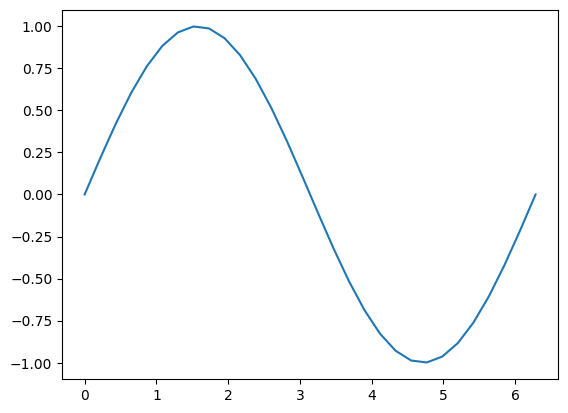
\includegraphics[width = \linewidth]{src/11_matplotlib/images/line_plot.png}
    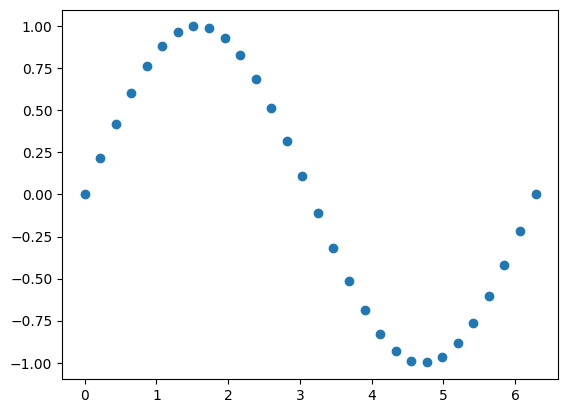
\includegraphics[width = \linewidth]{src/11_matplotlib/images/scatter_plot.png}
\end{minipage}

    \subsection{Histogram Plots}
To plot a histogram, use the following template:
\begin{minipage}{0.49\linewidth}
    \lstinputlisting{src/11_matplotlib/code/4_histogram.py}
\end{minipage}
\begin{minipage}{0.49\linewidth}
    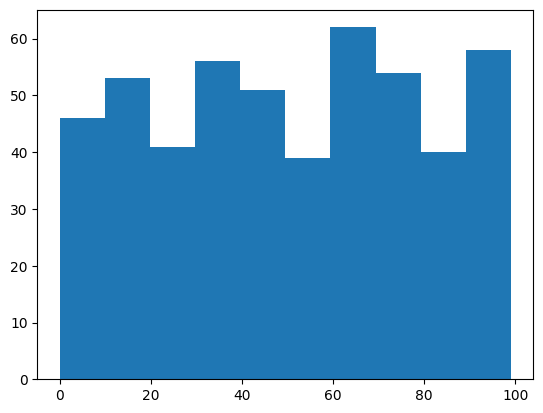
\includegraphics[width = \linewidth]{src/11_matplotlib/images/histogram_plot.png}
\end{minipage}


    \subsection{Graph Styling}
\lstinputlisting{src/11_matplotlib/code/5_styling.py}


\end{document}